%% Uses the local kiseon_memo document class (docs/kiseon_memo.cls), which
%% auto-loads graphicx, amsmath, amssymb, hyperref, xcolor, kotex, fancyhdr,
%% and sets its own geometry / boxed title / header-footer.  booktabs is not
%% provided by the class, so it is loaded here.
\documentclass{kiseon_memo}
\usepackage{booktabs}

\newcommand{\Rp}{R_{\mathrm{p}}}
\newcommand{\Mdot}{\dot{M}}
\newcommand{\EXHALE}{\textsc{Exhale}}

\title{Version comparison: \EXHALE\ v1.0 vs current (He/H $+$ metal diffusion)\\
on HD\,209458b and WASP-121b}
\author{K.-I. Seon}
\date{\today}

\begin{document}
\maketitle

\section{Purpose and setup}

Quantify what the new diffusive separation changes in \EXHALE's predictions, by running the
\emph{same} planet on two code versions, for \emph{two contrasting planets}:

\begin{itemize}
  \item \textbf{v1.0} (\texttt{ATES/EXHALE\_v1.0/}): clean GitHub \texttt{main} $+$ the
    temperature-dependent Penning rate. \emph{No} diffusive separation.
  \item \textbf{current} (\texttt{ATES/EXHALE/}): v1.0 physics $+$ He/H and per-element metal
    diffusion (\texttt{He\_diffusion} $+$ \texttt{He\_metal\_diffusion}, ambipolar on).
\end{itemize}

Both share the temperature-dependent Penning rate, so the only difference is the diffusion.
Setup: He\,2$^3$S on, trace metals from \texttt{metals.inp} (HD\,209458b: C/N/O; WASP-121b:
C/N/O/Mg/Ca/Na/Fe), identical \texttt{input.inp} per planet, 15000 relaxation steps.
Runs/figures/script: \texttt{docs/version\_compare/}.

\section{Headline numbers}

\begin{table}[h]
\centering
{\bfseries HD\,209458b (hot Jupiter, $\log_{10}\Mdot\approx9.3$ --- gentler escape)}\par
\vspace{3pt}
\begin{tabular}{lccc}
\toprule
quantity & v1.0 (no diff) & current (diff) & change \\
\midrule
He/H at 3\,$\Rp$ & 0.083 (flat) & \textbf{0.014} & $-83\%$ \\
peak $n$(He\,2$^3$S) [cm$^{-3}$] & 177 & 102 & $-42\%$ \\
\textbf{He\,I 10830 line-center absorption} & \textbf{70.5\%} & \textbf{27.2\%} & \textbf{$-2.6\times$} \\
$\log_{10}\Mdot$ [g\,s$^{-1}$] & 9.31 & 9.04 & $-0.27$ dex \\
\bottomrule
\end{tabular}

\vspace{10pt}
{\bfseries WASP-121b (ultra-hot Jupiter, $\log_{10}\Mdot\approx13.3$ --- furious escape)}\par
\vspace{3pt}
\begin{tabular}{lccc}
\toprule
quantity & v1.0 (no diff) & current (diff) & change \\
\midrule
He/H (min, 1.05--1.5\,$\Rp$) & 0.083 & \textbf{0.053} & $-36\%$ (weaker) \\
peak $n$(He\,2$^3$S) [cm$^{-3}$] & 3517 & 2383 & $-32\%$ \\
He\,I 10830 line-center absorption & 53.7\% & 53.6\% & $\sim$unchanged \\
metal/H (elem/base) & 1.0 & tracks He ($\sim$0.6--1.0; no extra fractionation) & none \\
$\log_{10}\Mdot$ [g\,s$^{-1}$] & 13.34 & 13.32 & unchanged \\
\bottomrule
\end{tabular}
\end{table}

\textbf{Two regimes.} On the gentler HD\,209458b the escape is slow enough that \emph{helium
itself} diffusively separates, cutting the He\,I 10830 line by $\sim$2.6$\times$, and the
heavier C/N/O deplete more than He aloft (He $>$ C $>$ N $>$ O at 3\,$\Rp$). On the furious
WASP-121b ($\sim$4 dex stronger wind) advection dominates settling for \emph{every} species
--- helium \emph{and} the metals are dragged out essentially unfractionated (10830 unchanged;
metal/H tracks He/H). This is the (settling speed)/(wind speed) scaling of Koskinen et al.\
(2013) / Xing et al.\ (2023): separation is suppressed by fast escape and, where it operates
at all, is stronger for heavier species.

\emph{Correction note: an earlier version showed WASP-121b metals collapsing to zero by
$\sim$1.25\,$\Rp$ (a ``metal homopause''). That was an artifact of two bugs in the metal
rescale --- an $r_X\le1$ clamp that made depletion a one-way ratchet, and a skip of exhausted
cells that made holes permanent --- which locked in transient early-relaxation settling
before the wind developed. With the fix, metals recover with the wind and track He, and the
v1-vs-v2 temperature structures agree; the earlier ``$\sim$2500\,K hotter'' claim is also
retracted.}

\section{HD\,209458b}

\begin{figure}[h]
\centering
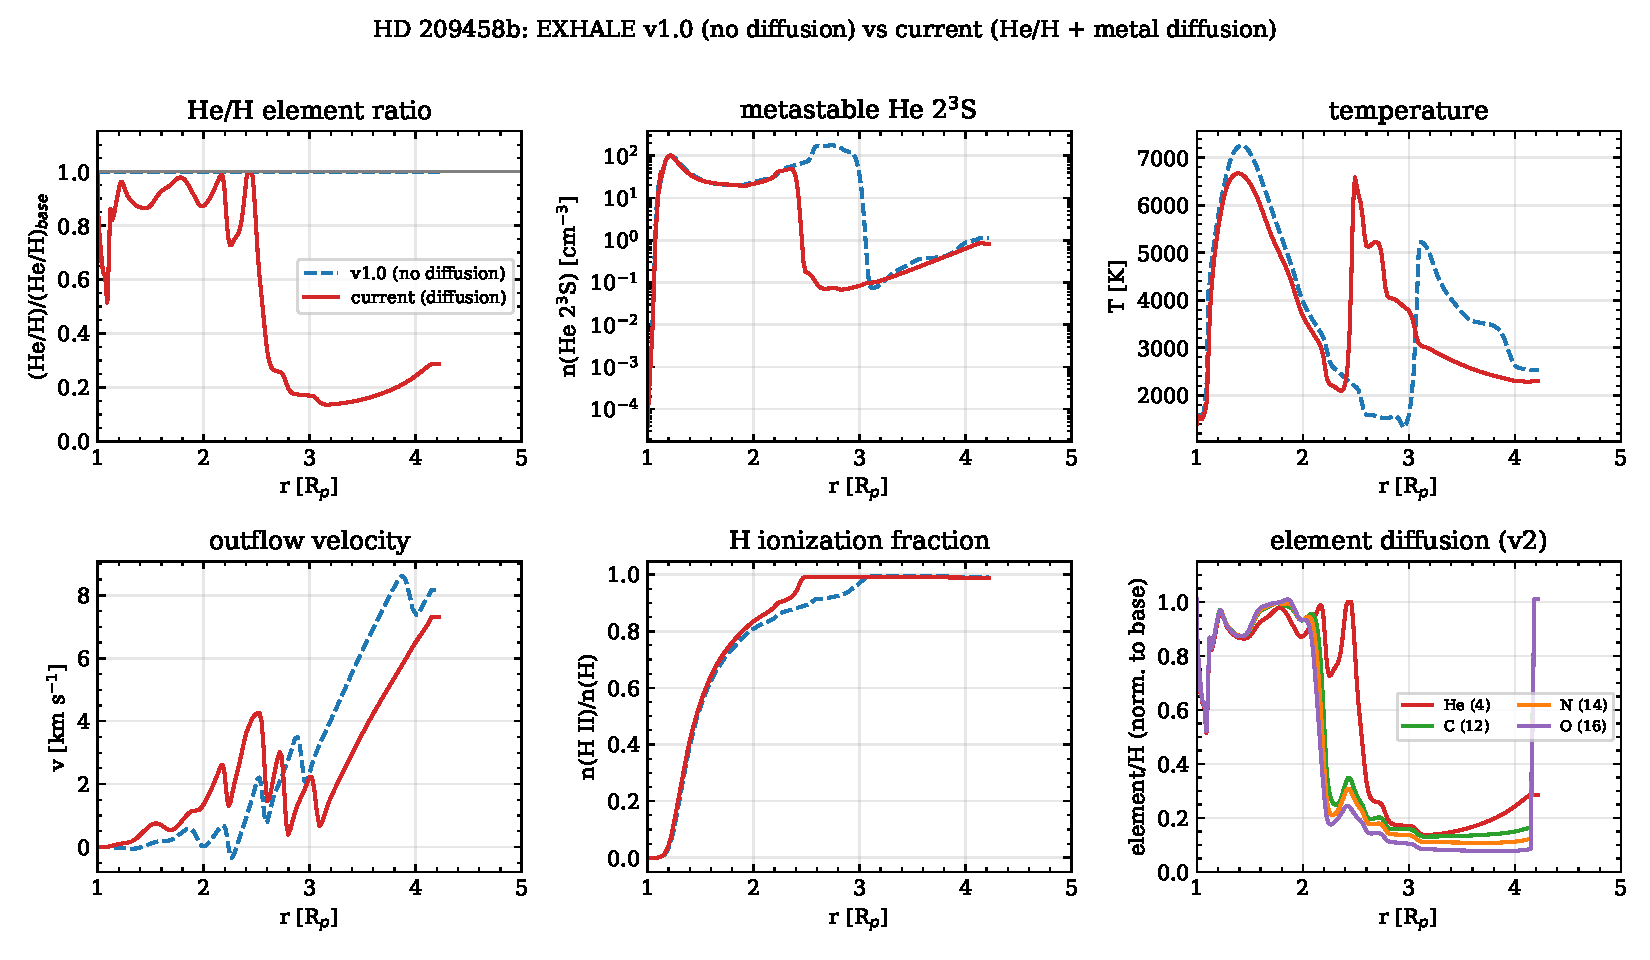
\includegraphics[width=\textwidth]{version_compare/fig_hd209_profiles.pdf}
\caption{HD\,209458b, v1.0 (blue dashed) vs current (red). He/H falls to $\sim$0.15--0.3$\times$
aloft; the He\,2$^3$S reservoir contracts. Bottom-right: C/N/O deplete more than He aloft
(mass ordering He $>$ C $>$ N $>$ O above $\sim$2.5\,$\Rp$).}
\end{figure}

\begin{figure}[h]
\centering
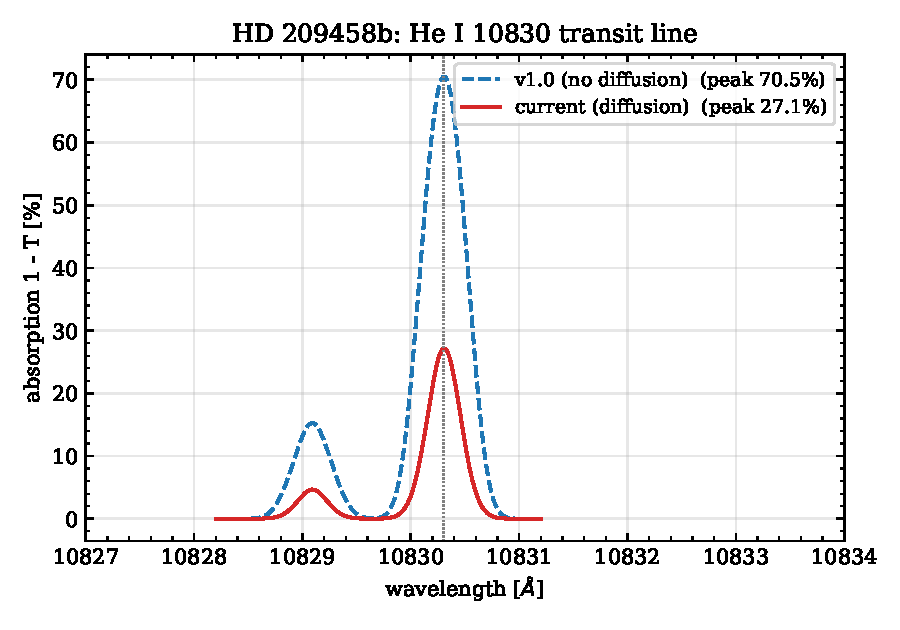
\includegraphics[width=0.66\textwidth]{version_compare/fig_hd209_He10830.pdf}
\caption{He\,I 10830 line: diffusion lowers the line-center absorption 70.5\%$\to$27.2\% and
narrows the profile.}
\end{figure}

\clearpage
\section{WASP-121b}

\begin{figure}[h]
\centering
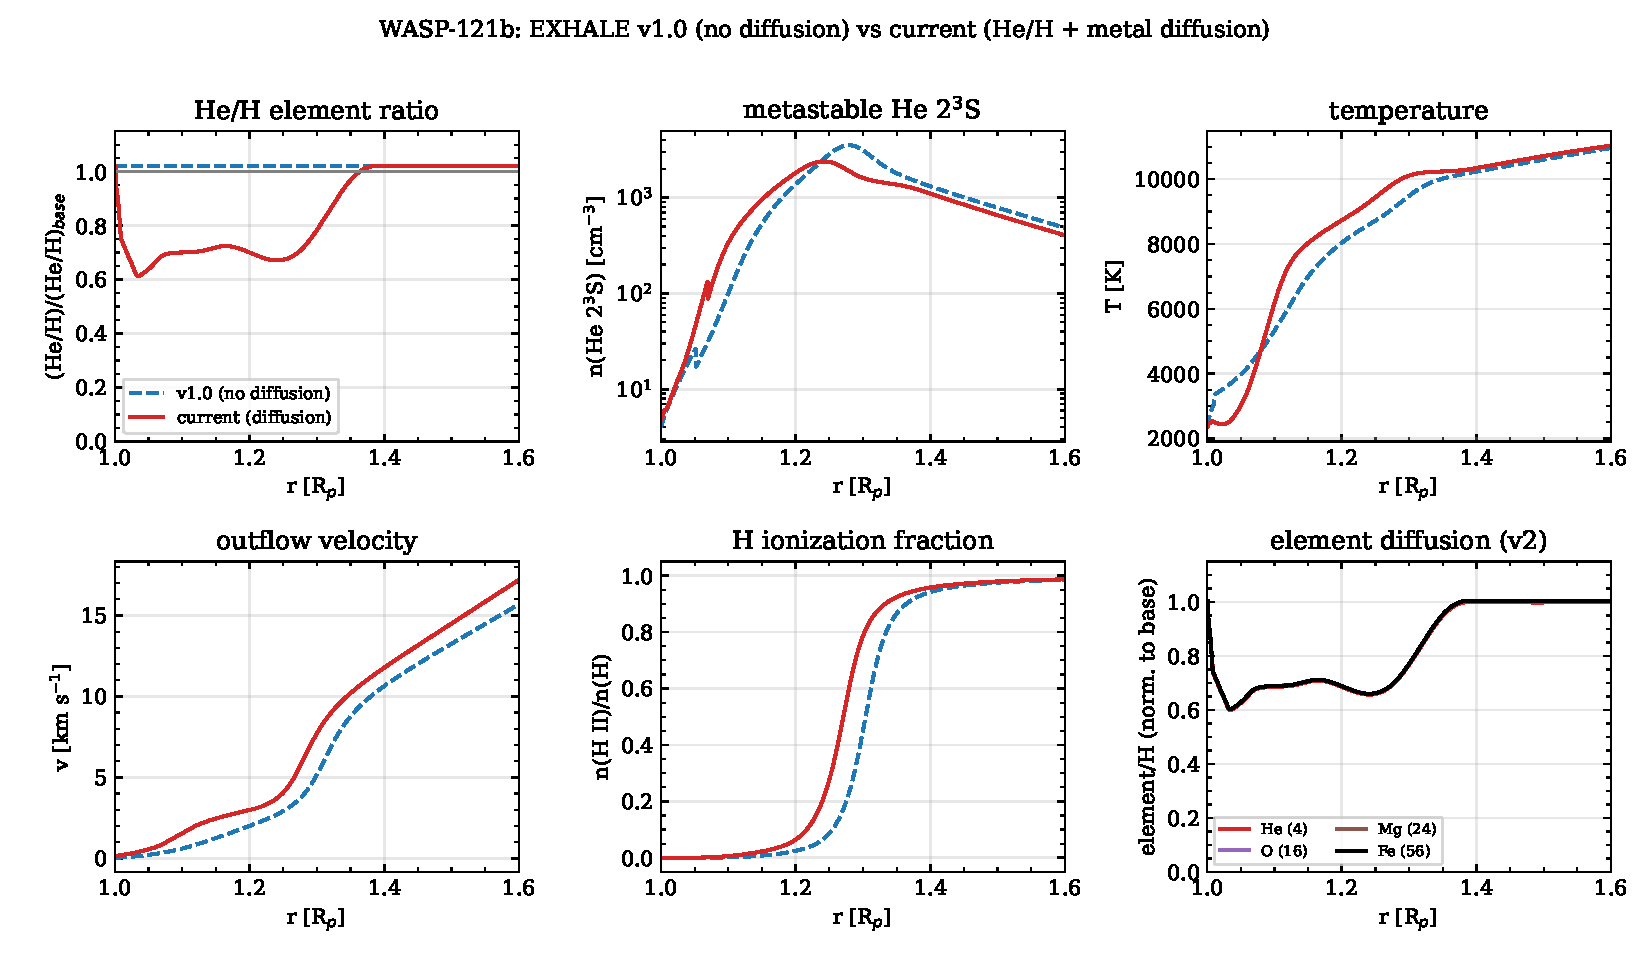
\includegraphics[width=\textwidth]{version_compare/fig_wasp_profiles.pdf}
\caption{WASP-121b (compact domain, escape radius 1.5\,$\Rp$). He/H separates only modestly
($\sim$0.6--0.75$\times$, returning to $\sim$1 above 1.4\,$\Rp$) because the
$\sim$4-dex-stronger wind drags helium out. The metals (O, Mg, Fe) overlap He almost exactly
--- even Fe (mass 56) is advection-dominated here, so no additional fractionation develops.
The v1/v2 temperature and velocity structures are nearly identical.}
\end{figure}

\begin{figure}[h]
\centering
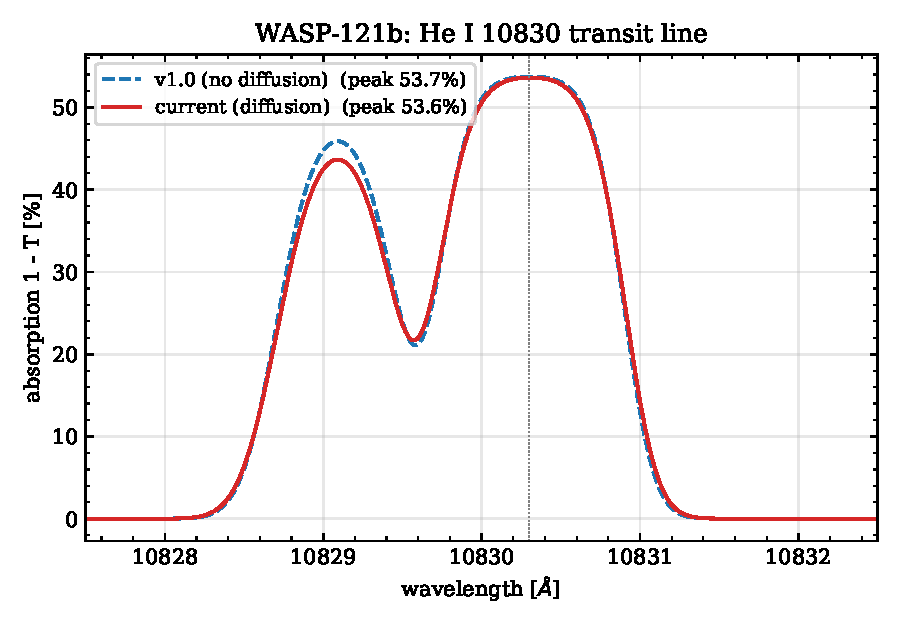
\includegraphics[width=0.66\textwidth]{version_compare/fig_wasp_He10830.pdf}
\caption{He\,I 10830 line: the core is essentially unchanged (53.7\%$\to$53.6\%) since helium
is not strongly separated in the line-forming region.}
\end{figure}

\clearpage
\section{Interpretation and caveats}

\textbf{Interpretation.}
\begin{itemize}
  \item \textbf{He/H.} On HD\,209458b settling competes with the slow wind, so He/H declines
    with altitude and 10830 weakens; on WASP-121b the wind is $\sim$4 dex stronger, so helium
    is dragged out nearly unfractionated.
  \item \textbf{He\,2$^3$S / 10830.} The metastable tracks He abundance --- weakened where He
    is depleted (HD\,209458b), preserved where He stays mixed (WASP-121b).
  \item \textbf{Metals.} Each trace metal diffuses independently with its own mass, binary
    $D$, and ambipolar-corrected settling. Where diffusion competes with the wind
    (HD\,209458b aloft) heavier elements deplete faster (He $>$ C $>$ N $>$ O); where
    advection dominates (WASP-121b) even Fe stays locked to He. Relevant for metal-line
    transmission (Mg\,II/Ca\,II/Na\,I in \texttt{TPM.py}).
\end{itemize}

\textbf{Caveats.}
\begin{itemize}
  \item \textbf{Absolute values uncalibrated.} The 27--70\% He 10830 depths far exceed
    observations ($\sim$1--2\%); heating efficiency / XUV / He\,2$^3$S microphysics were not
    tuned. The \emph{relative} change and the two-planet \emph{contrast} are the robust
    results.
  \item \textbf{Scheme / convergence sensitivity.} Step-capped (not Newton-finished), so
    $\Mdot$ is indicative; the He-separation magnitude is somewhat sensitive to the settling
    discretization (a Peclet-hybrid central/upwind scheme: central where well-resolved, upwind
    for the stiff heavy-metal settling).
  \item \textbf{Phase-1/2 numerics.} Mild non-monotonic structure from the He/H cap and the
    not-fully-developed wind; see \texttt{design\_hehe\_diffusion.md} \S7d--\S7e. Diffusion
    flags \textbf{default OFF}.
\end{itemize}

\end{document}
